\section{Sequenzielle Schaltung}
\textbf{Kombinatorische} Schaltungen sind Zustandsfrei. Ausgänge sind direkt von Eingängen abhängig.\\
\textbf{Sequenzielle} Schaltungen sind zustandsbehaftet (d.h. mehrere Zustände). Vergangenes Verhalten und Eingänge bestimmen momentanen Zustand und Ausgänge.

\subsection{Takt}
\begin{tabular}{ll}
	Periode & $T = T_{on} + T_{off}$ \\
	Frequenz &  $F = \frac{1}{T}$ \\
	DutyCycle &  $DutyCycle = \frac{T_{on}}{T}$ \\
\end{tabular}

\subsection{Synchron/Asynchron}
Bei \textbf{Synchron} wechselt der Zustand bei einer Flanke des Clocks statt.\\
Bei \textbf{Asynchron} kann der Zustand zu jeder Zeit statt finden.

\subsection{Hardware Grundelemente}
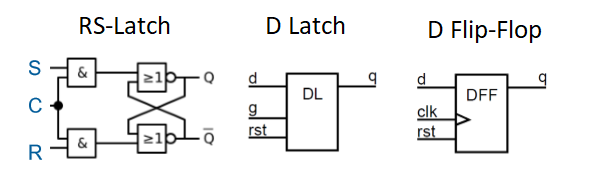
\includegraphics[width=\columnwidth]{./Images/FlipFlops.png}

\subsection{Timing Diagram - Längster Pfad}
\begin{minipage}{\columnwidth}
	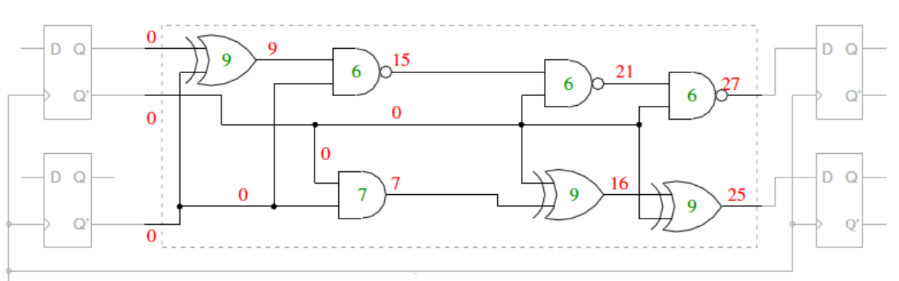
\includegraphics[width=\columnwidth,keepaspectratio=true]{./Images/pfad.png}\\
	Eingänge mit $0$ beschriften, anschliessend recursive alle Ausgänge = $\max\{\text{Eingänge}\} + t_p$. Der längste Pfad ist $\max\{\text{Eingänge}\}$.
\end{minipage}